\section{Rekonštrukcia}

Táto časť sa bude venovať zostavovaniu opravovaného čítania z jadier korekcie pomocou grafu popísaneho v predchádzajúcej podkapitole. Silné jadrá korekcie tu zohrávajú veľmi podobnú funkciu ako silné $k$-tice v nástroji LoRDEC. Najprv nájdeme cesty v grafe prepájajúce blízke jadrá korekcie s čo najnižšou editačnou vzdialenosťou od sekvencie na čítaní medzi danými silnými jadrami. V druhej fáze budeme hľadať podpostupnosť silných jadier korekcie s najnižším súčtom editačných vzdialeností prepájajúcich ciest.

\subsection{Hľadanie najlepšej cesty}

Na hľadanie cesty medzi dvomi silnými jadrami s najnižsou editačnou vzdialenosťou od pôvodnej sekvencie používame Dijkstrov algoritmus. Priestor pozícií je kartézsky súčin pozícií na opravovanom čítaní, všetkých jadier a všetkých pozícií v rámci jadier. Hľadanie cesty začína na konci ľavého silného jadra a jeho zodpovedájúcej pozícii v čítaní. Algoritmus skončí na ktorejkoľvek pozícii pravého silného jadra, ak pozícia v rámci čítania súhlasí s pozíciou tohto jadrá na čítaní. To, na ktorej pozícii v pravom jadre skončíme, nijako neovplyvňuje editačnú vzdialenosť.

\begin{figure}
    \centering
    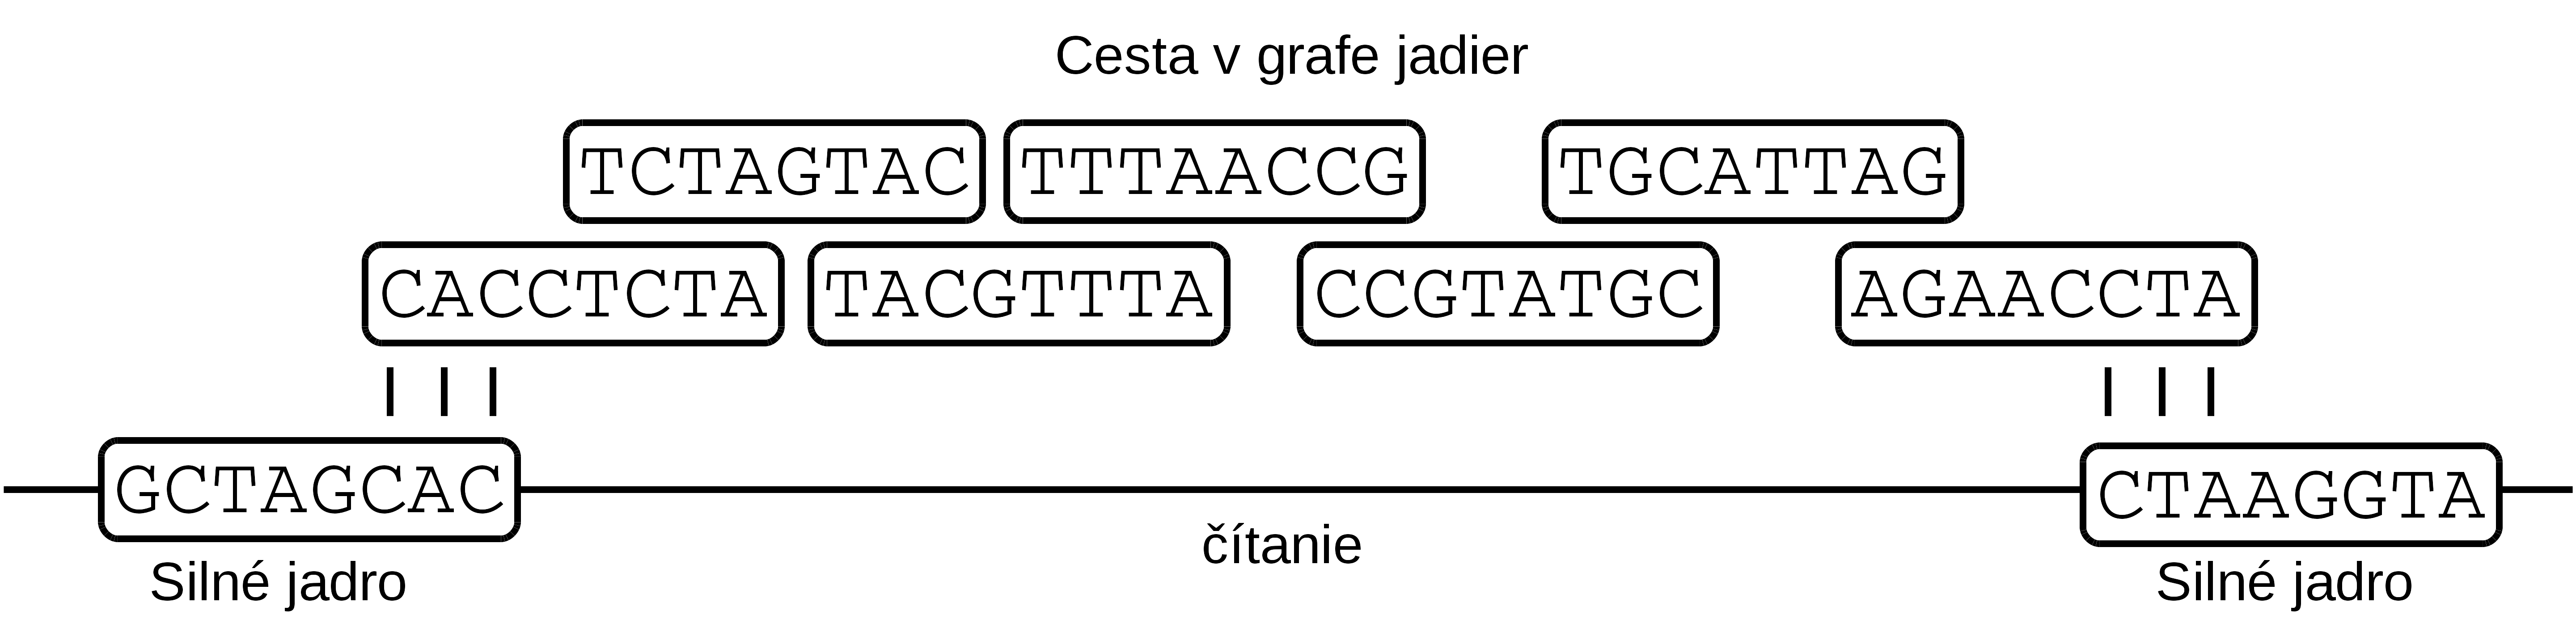
\includegraphics[width=0.9\textwidth]{images/recreating_path.png}
    \caption{Ukážka cesty v grafe jadier medzi dvomi silnými jadrami}
    \label{fig:recreating_path}
\end{figure} 

V každkej iterácii Dijkstrovho algoritmu môže nastať jedna z možností:
\begin{enumerate}[label={S.\arabic*}]
\item \label{na_konci_jadra} Nachádzame sa na konci jadra (za poslednou bázou)
\item \label{uprostred_jadra} Nachádzame sa niekde uprostred jadra
\end{enumerate}

V prípade \ref{na_konci_jadra} potrebujeme na predĺženie generovanej cesty prejsť na iné jadro korekcie. Do prioritného radu Dijkstrovho algoritmu pridáme nové pozície podľa hrán v grafe jadier. Pozícia na čitaní sa nezmení a pozícia na jadre, na ktoré sme preskočili, závisí od dĺžky prekrytia jadier. Tútu informáciu máme uloženú spolu s hranou v grafe.

V prípade \ref{uprostred_jadra} rozlišujeme podobne ako pri zarovnávaní sekvencií štyri možnosti:

\begin{enumerate}[label={R.\arabic*}]
\item \label{item:zhoda}        Zhoda -- ak na čítaní nasleduje rovnaká báza ako na jadre, algoritmus pridá do prioritného radu pozíciu o jednu bázu posunutú na čítaní aj jadre. Editačná vzdialenosť tejto pozície je rovnaká, takže túto pozíciu pridáme akoby na začiatok radu.
\item \label{item:inzercia}     Inzercia -- na tento druh chyby čítania sa pozeráme z pohľadu výslednej sekvencie. Ide o prípad, kedy je v čítaní báza navyše oproti sekvencii jadra. Algoritmus vytvorí pozíciu, ktorá je posunutá na čítaní oproti východzej pozícii, ale na jadre sa neposunie. 
\item \label{item:delecia}      Delécia -- opačný prílad ako inzercia. Algoritmus sa posunie len na jadre.
\item \label{item:substitucia}  Substitúcia -- kedže sekvenačne zariadenie niekedy urobí aj tento druh chyby, dovolíme aj nášmu algoritmu \''zarovnať\'' na seba rôzne bázy. Postup je podobný ako pri zhode, ale editačná vzdialenosť novej pozície je penalizovaná.
\end{enumerate}

Ak nastane zhoda, môžeme v snahe minimalizovať zbytočné vetvy výpočtu nebrať do úvahy ostatné možnosti. Dá sa nahliadnuť, že pri rozumných nastaveniach penalizácie toto obmedzenie nijako nezhorší editačnú vzdialenosť nájdenej cesty. Podobné orezanie vetiev sa dá urobiť pri prechádzaní z jedného jadra na druhé. Ak z jadra smeruje hrana s prekrytím $k - 1$ a pridaná báza sa zhoduje s bázou, ktorá nasleduje na čítaní, ostatné hrany nepoužijeme. Toto zrýchlenie za istých okolností môže negatívne ovplyvniť výsledok. V nasledujúcej kapitole otestujeme ako vplýva na kvalitu výsledného zarovnania a rýchlosť výpočtu.

\subsubsection{Penalizácia}

Penalizácia v našom algoritme je analógiou skórovacieho systému pri zarovnávaní sekvencií. Penalty sa používajú ako vzdialenosti medzi pozíciami v priestore pozícií Dijkstrovho algoritmu. Programu je možné nastaviť rôzne penalty pre inzerciu, deléciu a substitúciu. %Chyby vznikajúce sekvenáciou zariadením PacBio RS II sú prevažne inzercie a preto je vhodné tento druh chyby penalizovať menej ako ostatné. Vplyv rozdielu penalizácie medzi inzerciou a ostatnými otestujeme v nasledujúcej kapitole. 

Penalizáciu vieme využiť aj na dosiahnutie čo najvačších prekrytí po sebe idúcich jadier v hľadanej ceste. Krátke prekrytia sú nebezpečné, lebo vo vačšine prípadov vznikli náhodou a umožnia tak vytvoriť nesprávne sekvencie. Ak dosiahneme vysoké priemerné prekrytie jadier, jednotlivé bázy budú ležať na viacerých jadrách, čo zvyšuje ich dôveryhodnosť. Pri prechádzaní z jadra na iné jadro preto algoritmus udeľuje penaltu vo výške danej nejakou funkciou s parametrom veľkosti prekrytia. Vyskúšali sme použiť lineárne aj kvadratické funkcie.

Pri vytváraní grafu jadier sme obmedzili očakávanú vzdialenosť medzi prepojenými jadrami. Avšak, viacero nešťastných krokov po sebe môže spôsobiť, že jadro korekcie použijeme niekde úplne inde, ako by sa malo nachádzať. Podobne ako s veľkosťami prekrytí vieme toto zlé umiestnenie penalizovať. Treba však zobrať do úvahy, že pozície jadier sú len odhadované a malé rozdiely nič neznamenajú. Nastavíme preto pevnú hranicu, a ak su vzdialenosť použitia jadra na čítaní od očakávanej pozície prekročí, udelí sa za to konštantná penalizácia.

\subsection{Heuristiky}

V nasledujúcom texte popíšeme heuristické metódy na urýchlenie procesu hľadania ciest medzi silnými jadrami. Cieľom je zamedziť prehľadávanie vetiev, ktoré sú s vysokou pravdepodobnosťou nesprávne. Celý prehľadávaný priestor má $|r||V|k$ pozícií, kde $|r|$ je dĺžka úseku čítania medzi dvomi jadrami korekcie, $|V|$ je počet jadier a $k$ je dĺžka jadier. Úlohou heuristík je znížiť počet prehľadaných pozícií na čo najmenší násobok $|r|$, a teda aby bol čas výpočtu lineárne závislý len od dĺžky úseku.

\subsubsection{Vzdialenosť od najlepšej cesty}

V algoritme je editačná vzdialenosť po sebe vyhodnocovaných pozícií neklesajúca, ale pozícia na čítaní by môže skákať po celom opravovanom úseku. Vetvy, ktoré sú viac vpredu oproti ostatným majú na dovtedy opravenej ceste vačší počet zhôd. Výpočet zrýchlime tým, źe zahodíme vetvy, ktoré zaostávajú za najďalej siahajúcou vetvou o príliš vela miest. Princíp tejto metódy je podobný ako odstraňovanie vetiev výpočtu so zaostávajúcou antidiagonálou v nástroji DALIGN. 

\subsubsection{Lokálna kvalita cesty}

Cesty s vysokou mierou zhody a preto aj s náskokom v pozícii na čítaní majú tendenciu vytvárať nesprávne odbočky. Tieto odbočky spomaľujú napredovanie po čítaní a predchádzajúca heuristika ich odstráni až po niekoľkých iteráciách. Využijeme heuristikú metódu inšpirovanú nástrojom DALIGN. Pre každú pozíciu výpočtu si v bitovom vektore udžiavame zhody za posledných niekoľko báz cesty. Vetvy, ktoré majú počet zhôd menší ako zvolená hranica, sa zahodia. Môže spôsobiť, že sa cesta vôbec nenájde a to hlavne v prípadoch, keď nie celé čítanie je pokryté jadrami korekcie. 


Obe uvedené metódy môžu viesť k urýchleniu výpočtu a zároveň aj k zhoršeniu výsledných sekvencii. Na voľbu správnych parametrov sa pozrieme v ďalsej kapitole.

\subsection{Zostavenie výslednej sekvencie}

Zostáva už len naspať poskladať celé čítanie z vypočítaných úsekov medzi silnými jadrami. Doteraz sme neuviedli, medzi ktorými dvojicami silných jadier bude algoritmus hľadať cesty. Musí brať do úvahy, že aj silné jadrá korekcie nemusia byť správne. Zoberme situáciu, že máme tri neprekrývajúce sa silné jadrá A, B, C v uvedenom poradí a B je chybné. Dobre nastavená penalizácia by mala spôsobiť, že cesta z A do C má nižsiu editačnú vzdialenosť ako súčet editačných vzdialeností ciest z A do B a z B do C. 

Na zostavovanie výslednej sekvencie sa dá pozrieť ako na problém: Ako prejsť cez čítanie po silných jadrách, aby súčet editačných vzdialeností ciest po sebe idúcich silných jadier bol čo najmenší? Aby počet hľadaných ciest nebol kvadraticky závislý od počtu jadier, obmedzíme počet ''preskočených'' jadier konštantou $s$. Hľadaných ciest môže byť najviac $s|V|$, kde $|V|$ je počet jadier.

Na riešenie uvedeného problému použijeme dynamické programovanie. Algorimus postupne zľava do prava pre všetky silné jadrá počíta s akým najmenším možnym súčtom editačných vzdialeností sa dá do daného jadra dostať. Označme $N[i]$ najmenší súčet editačnych vzialeností cesty do $i$-teho silného jadra a $M[i, j]$ editačnú vzdialenosť prepojenia medzi $i$-tym  a $j$-tym silným jadrom. Platí, že $N[i] = min \{N[i - 1] + M[i - 1, i], ..., N[i - s - 1] + M[i - s - 1, i]\}$. Nenájdenie cesty medzi silnými jadrami môže spôsobiť, že niektoré hodnoty $N$ sú nedefinované. Ak pre nejaké $i$ sú všetky hodnoty $N[i - 1], ..., N[i - s - 1]$ nedefinované, nastavíme $N[i] = 0$ a považujeme toto jadro za začiatok dalšej opravujúcej sekvencie. Spätným prechodom hodnôt $N$ nájdeme všetky opravujúce sekvencie čítania.